
\section{VCS: Version control Systems}

\begin{frame}[fragile]{Keeping track of versions}

Either alone or in a team, one main problem of software development is \textit{keeping
track of changes} on the source code.

\vspace{1em}

\textbf{Why?}
\begin{itemize}
\item Complex projects/documents, built up over time
\item Multiple collaborators
\item Multiple (parallel) versions (eg. testing a new algorithm while the main
\textit{branch} of development is focused on other things)
\item Reproducibility (eg. bug hunting, etc.)
\end{itemize}
\end{frame}

\begin{frame}[fragile]{How do we track the code? Manual copies!}

\begin{center}

\includegraphics[height=0.89\textheight]{phd101212s}
\end{center}

\end{frame}

\begin{frame}[fragile]{How do we track the code? Manual copies!}

\begin{center}
\Huge NO!
\end{center}

Why?
\begin{itemize}
  \item Manual = fallible
  \item Labelling issue
  \item No metadata (dates, authors, etc.)
  \item No integrated/automated tool
\end{itemize}

\end{frame}

\begin{frame}[fragile]{How do we track the code? Dropbox/Google Drive/OneDrive!}

What about... \textbf{Dropbox/Google Drive/OneDrive}??

\end{frame}

\begin{frame}[fragile]{How do we track the code? Dropbox/Google Drive/OneDrive!}

\begin{center}
\Huge NO!
\end{center}

\normalsize
Why?
\begin{itemize}
  \item No concept of ``consistent checkpoint/commit"
  \item Collaboration is broken (unless you're working on very simple projects)
  \item No \textit{branching}/\textit{merging} capabilities
  \item Few metadata
  \item Too generic
\end{itemize}

\end{frame}

\begin{frame}[fragile]{How do we track the code? Version Control Systems!}

\begin{center}

\includegraphics[width=5em]{git-logo}
\hspace{10em}

\includegraphics[width=5em]{subversion-logo}
\end{center}

\begin{itemize}
  \item Consistent checkpoints, with \textbf{atomic operations}
  \item Written for text files (eg. source code), not for generic files
  \item Collaboration is well supported, eg. with file locking
  \item \textit{Branching}/\textit{merging} capabilities
  \item Metadata, a lot of
\end{itemize}

\end{frame}


\section{VCS: operations}

\begin{frame}[fragile]{VCS: components}

\begin{itemize}
  \item \textbf{Commit}: a ``snapshot" of the repository in a specific moment in time
  \item \textbf{Branch}: a parallel development
  \item \textbf{Merge}: the action of \textit{fusing} two branches in one
\end{itemize}

\end{frame}


\begin{frame}[fragile]{VCS: history}

\begin{center}
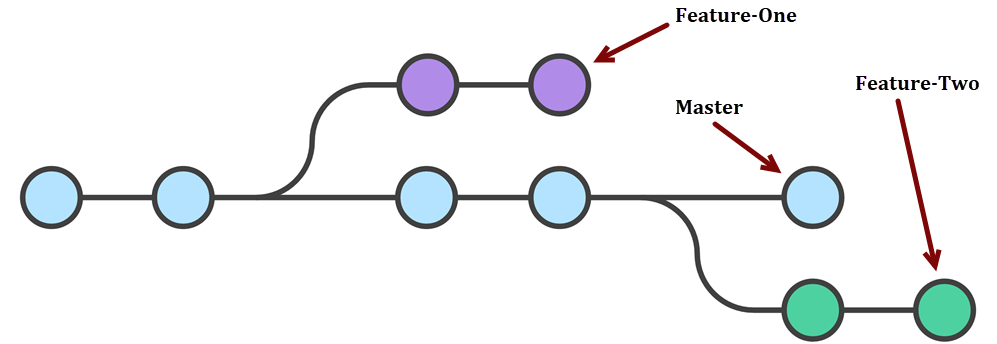
\includegraphics[width=\textwidth]{vcs-history}
\end{center}

\end{frame}


\begin{frame}[fragile]{VCS merge - fast forward}

\begin{center}
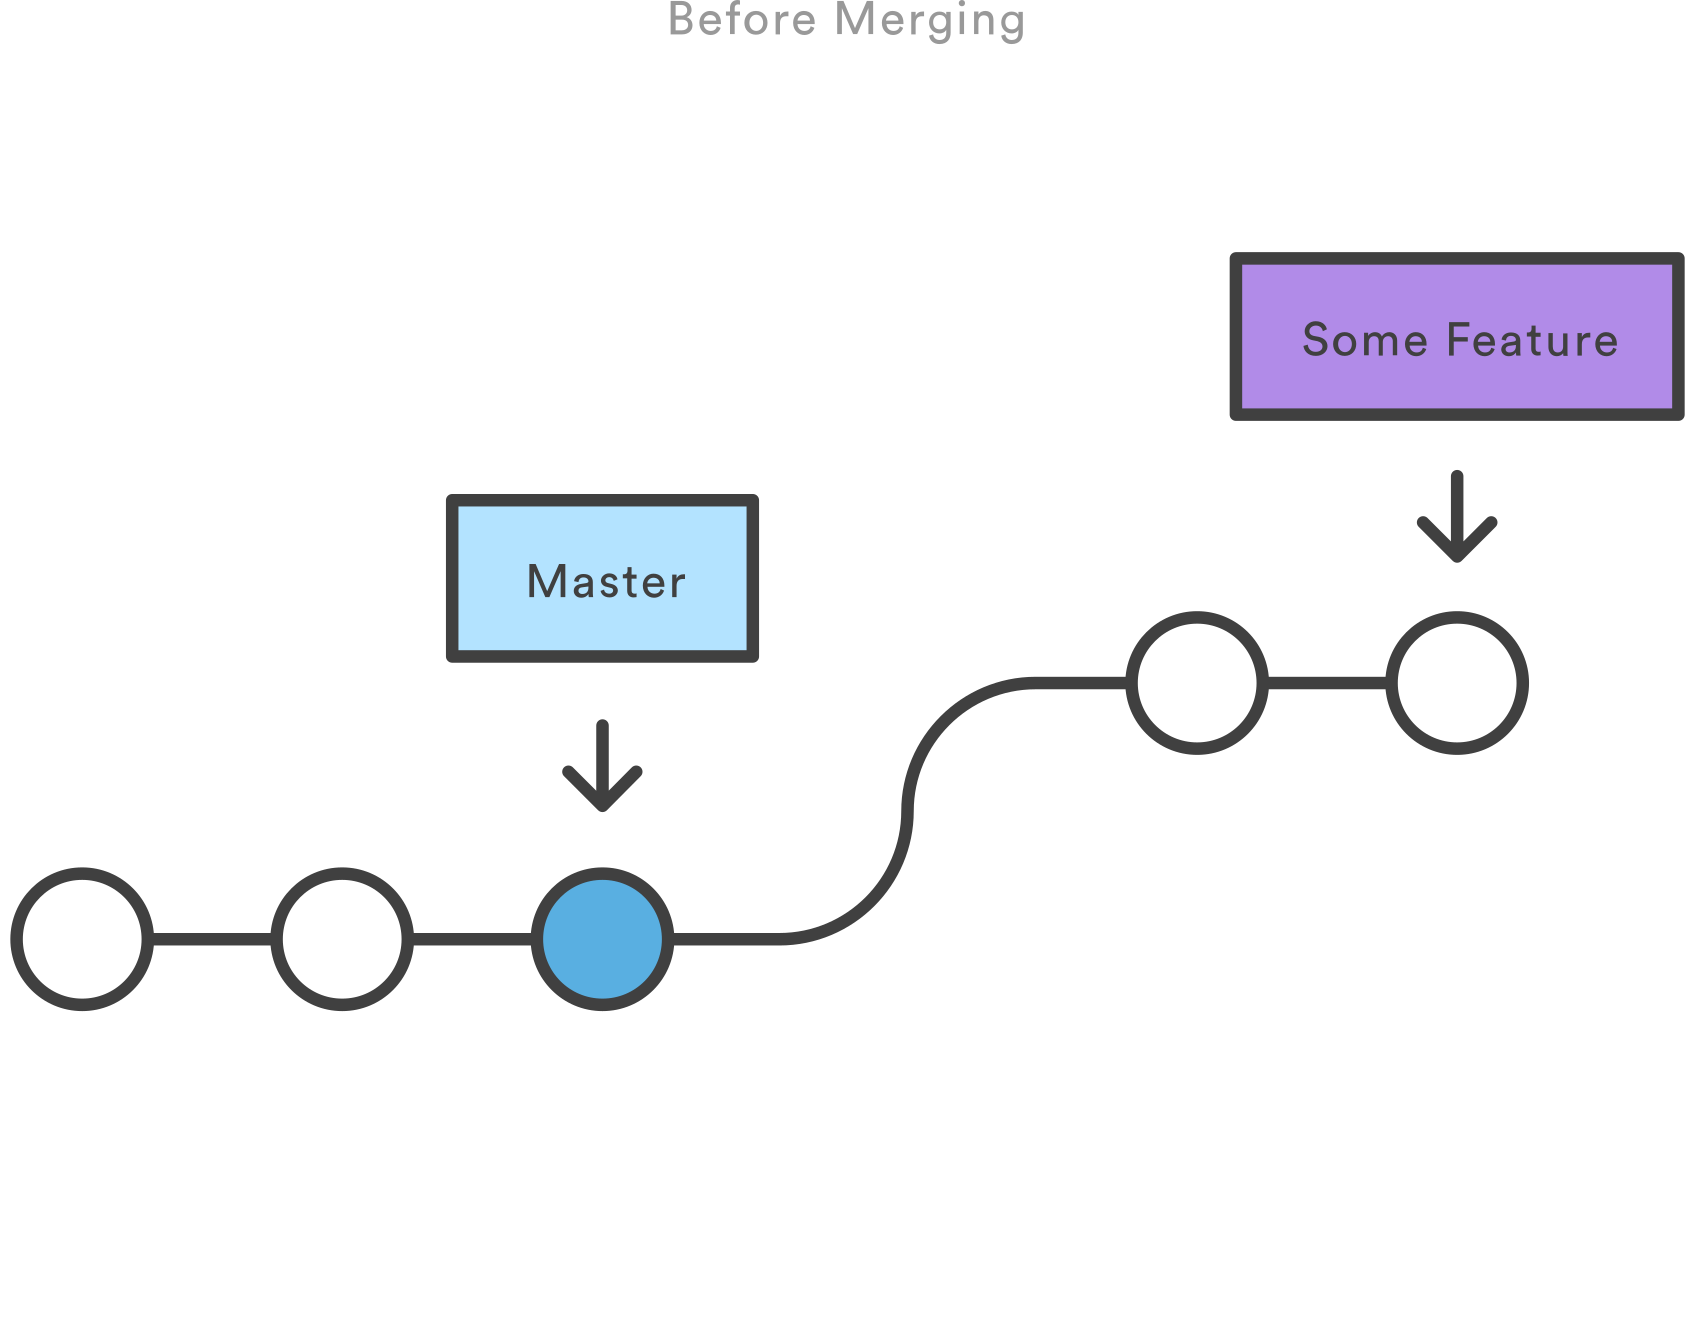
\includegraphics[width=\textwidth]{git-merge-ff}
\end{center}

\end{frame}


\begin{frame}[fragile]{VCS merge - fast forward}

\begin{center}
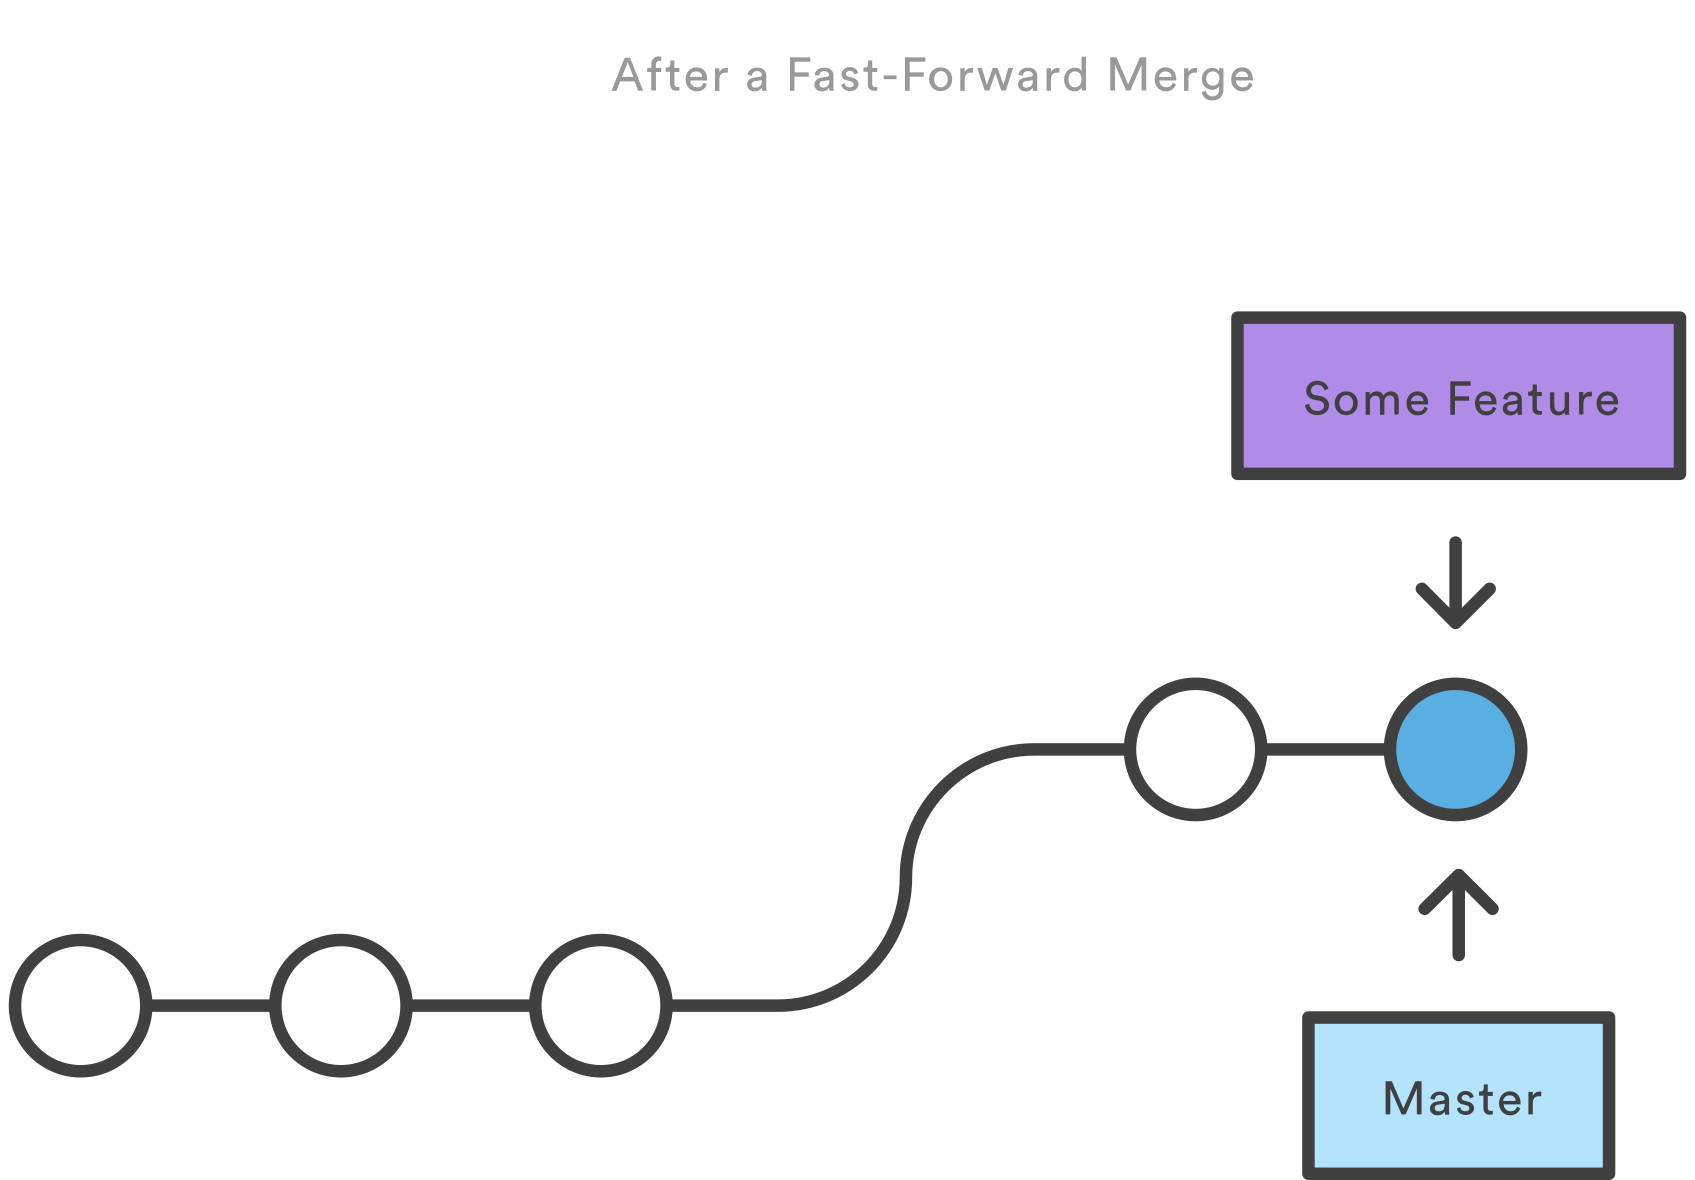
\includegraphics[width=\textwidth]{git-merge-ff2}
\end{center}

\end{frame}


\begin{frame}[fragile]{VCS merge - classic}

\begin{center}
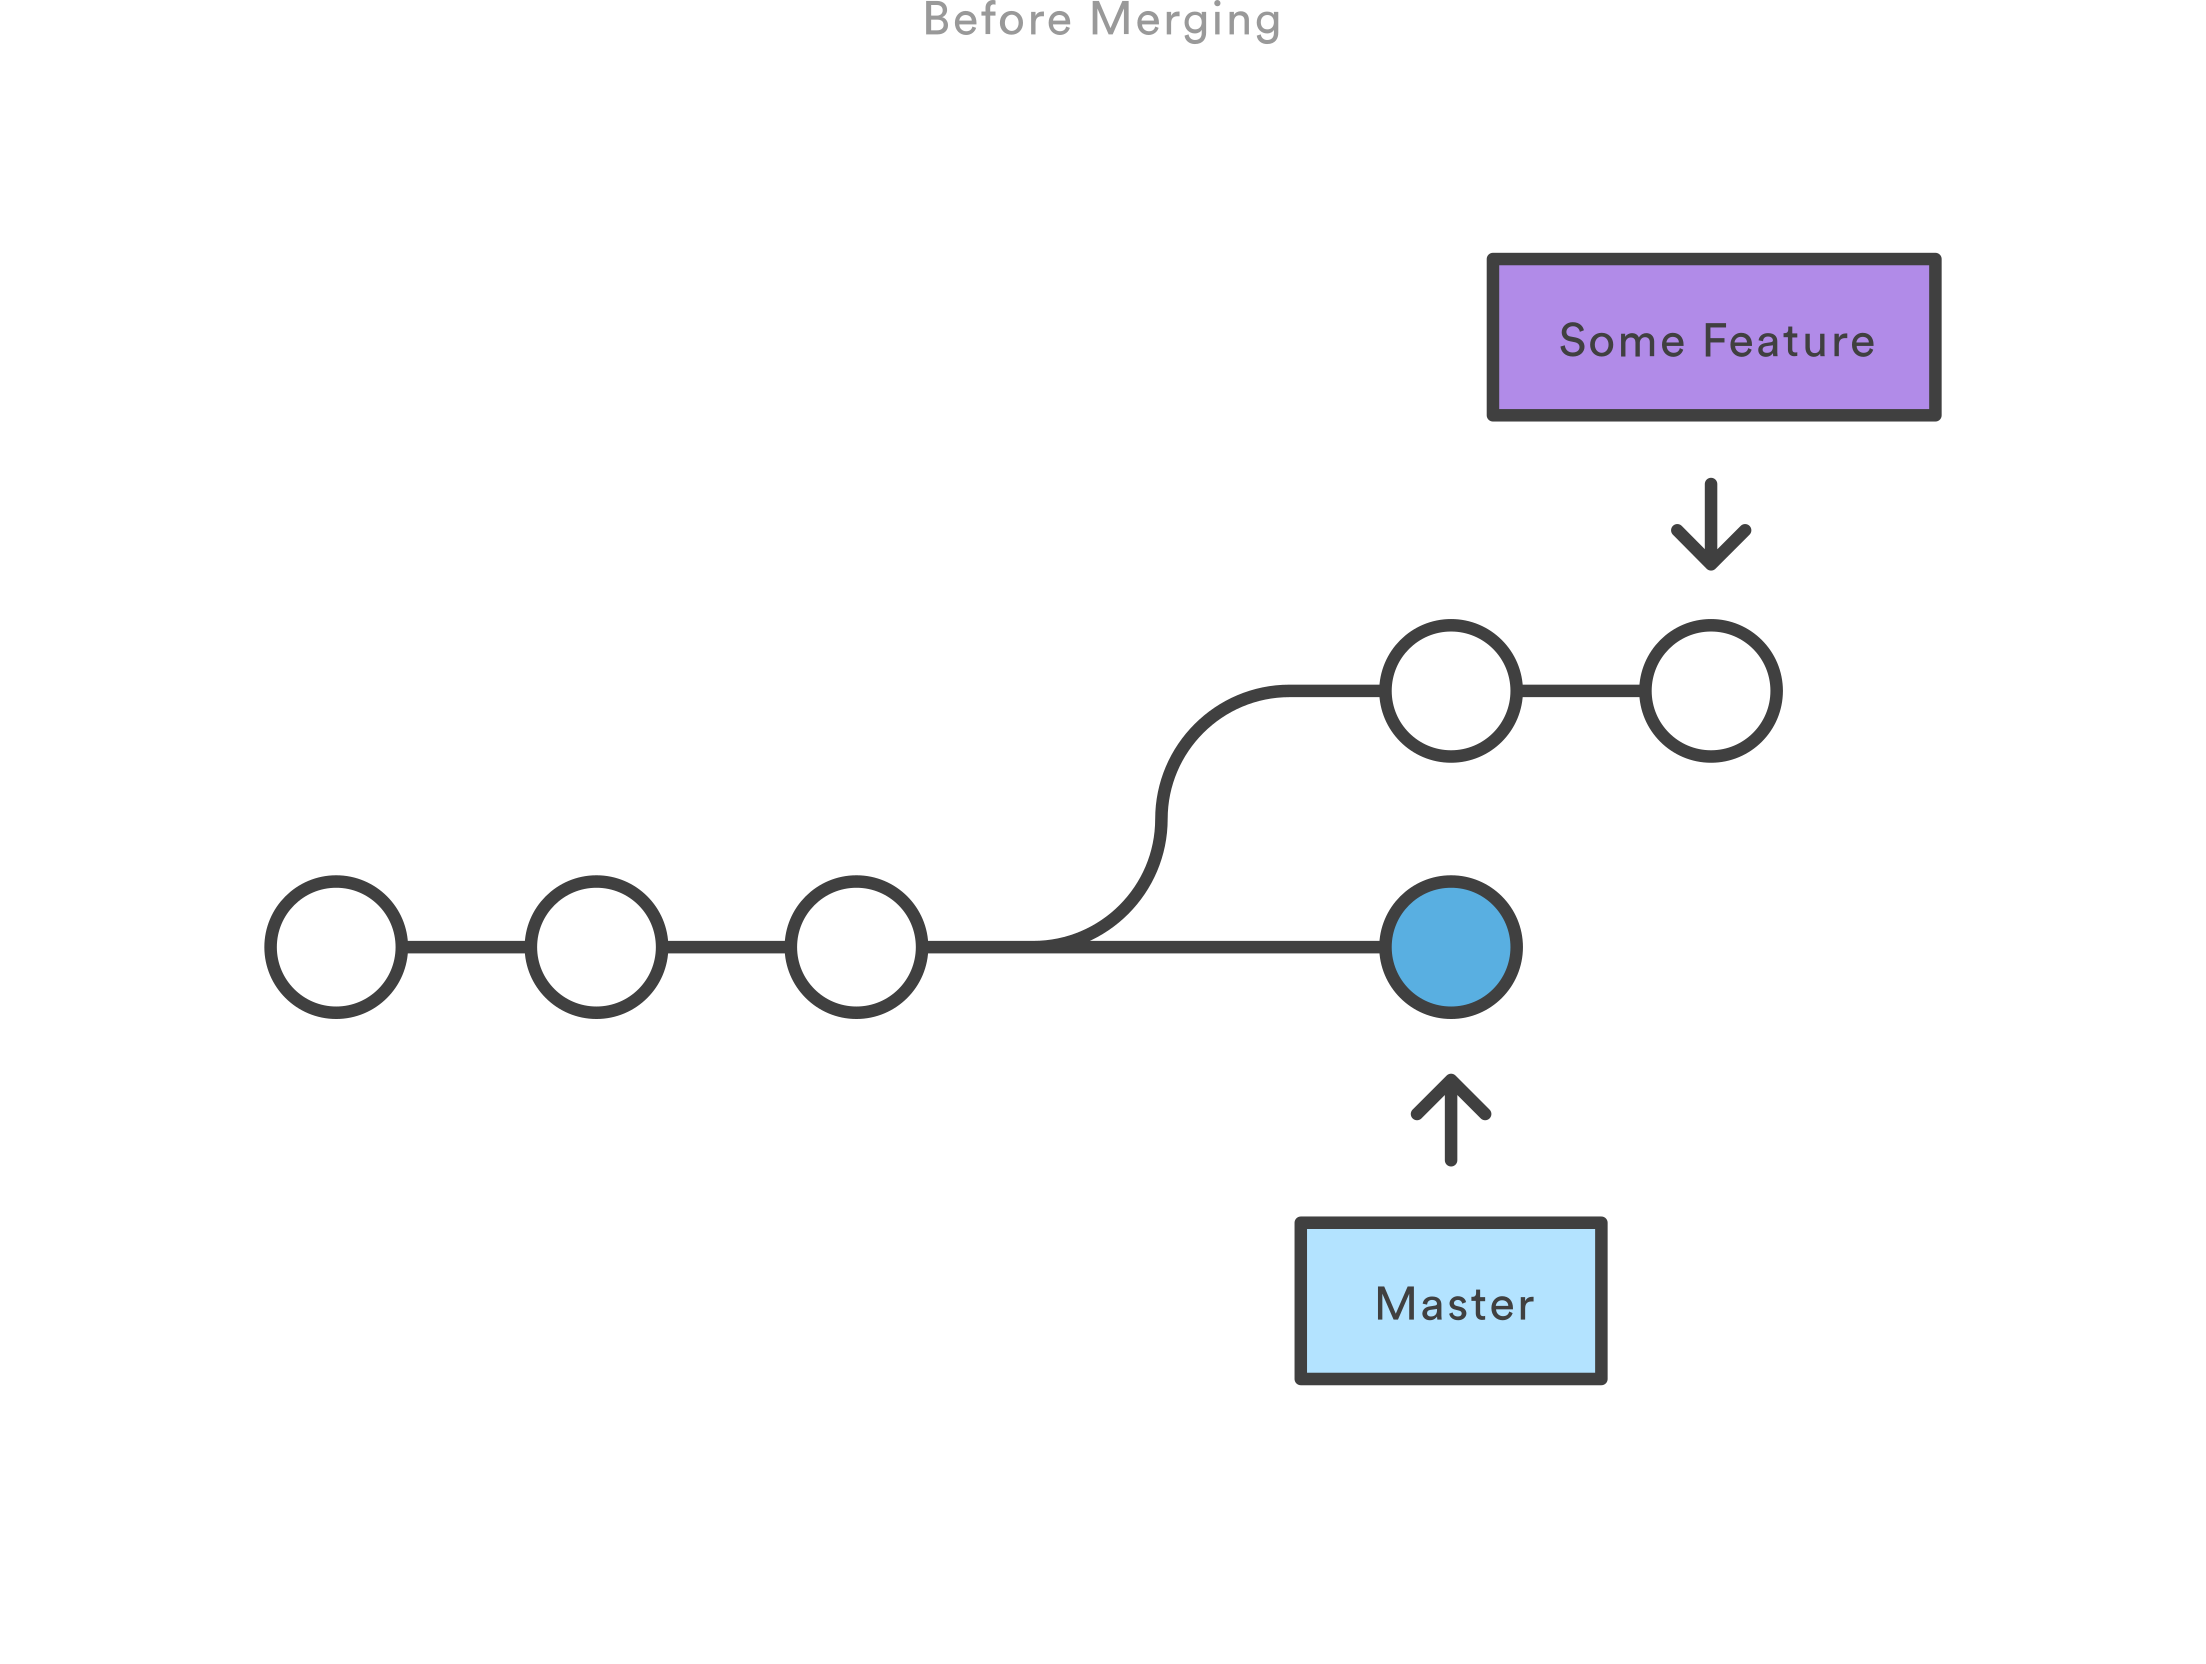
\includegraphics[width=\textwidth]{git-merge-nff}
\end{center}

\end{frame}

\begin{frame}[fragile]{VCS merge - classic}

\begin{center}
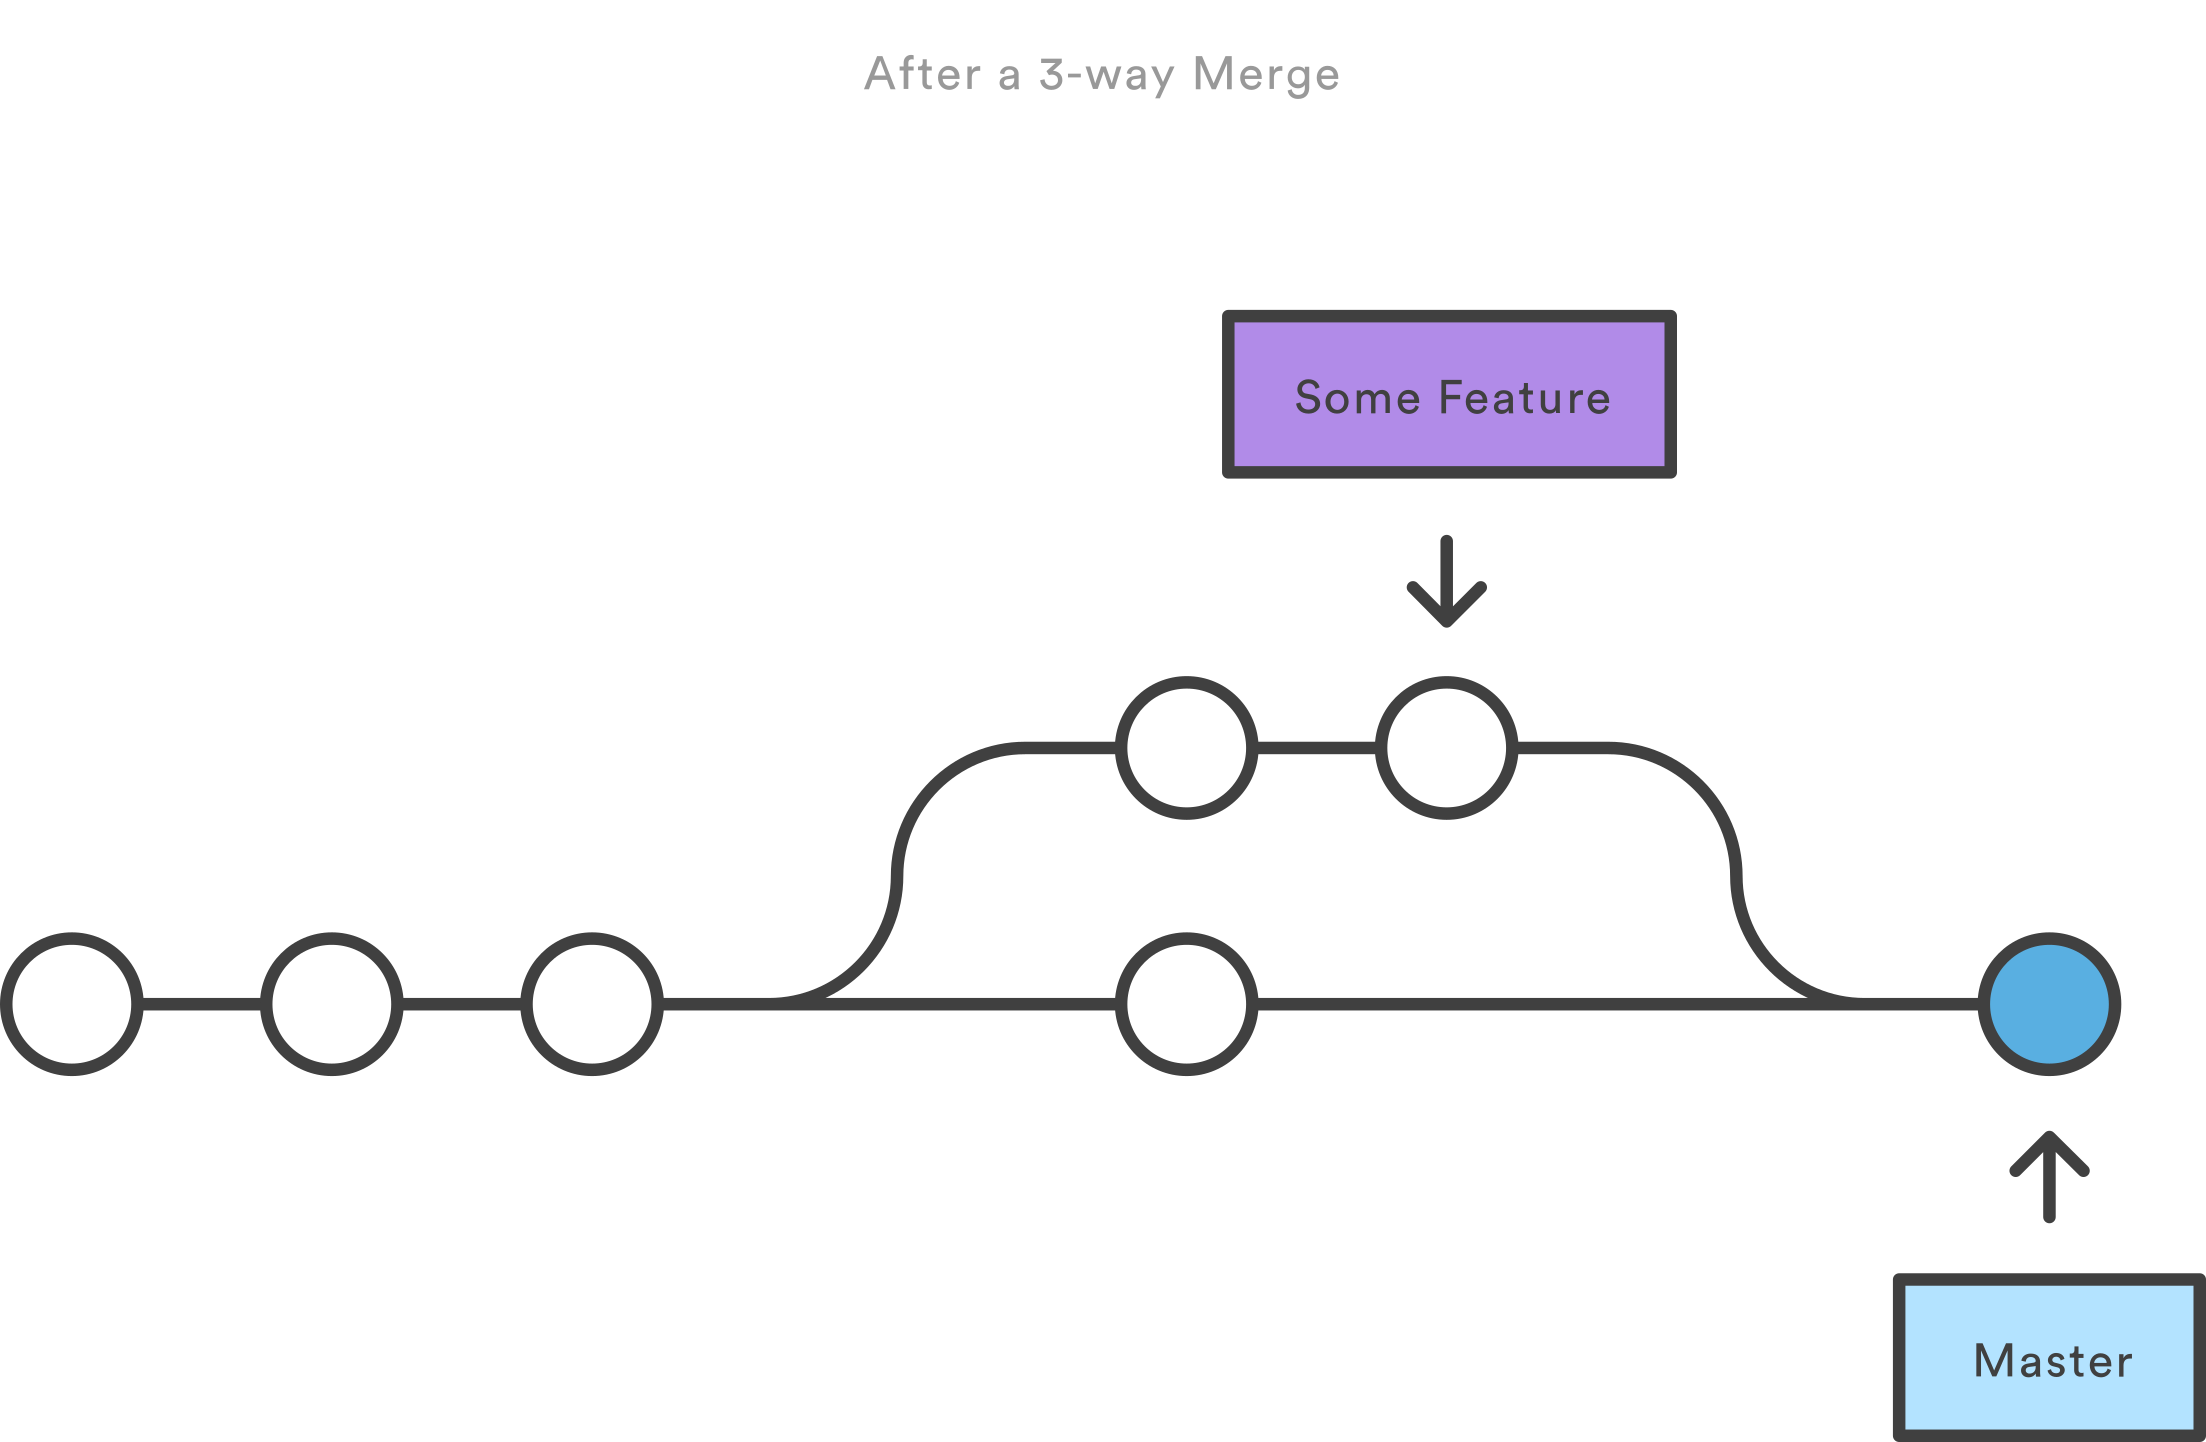
\includegraphics[width=\textwidth]{git-merge-nff2}
\end{center}

\end{frame}
